\documentclass[../main.tex]{subfiles}

\begin{document}
\chapter{Konstruktion der Reellen Zahlen}
\section{Historische Motivation}
In der Antike war Mathematik praktisch synonym mit Geometrie. Der Zahlenbegriff war
direkt an das Konzept der \textit{Länge} gekoppelt.

\begin{definition}[Euklid, 300 vor Christus]
  Zwei Längen $a,b > 0$ heissen \textit{kommensurabel}, falls eine Länge $L>0$ existiert,
  so wie zwei natürliche Zahlen $m,n \in \mathbb N$, so dass $a = mL$ und $b=nL$.
\end{definition}

Hier ist
\[\mathbb N = \{0, 1, 2, 3, 4, \dots\}\]
die Menge der Natürlichen Zahlen.

\begin{theorem}[Euklid]
  Die Seite und Diagonale eines ebenen Quadrats sind nicht kommensurabel.
\end{theorem}

\begin{proof}
  Dieser Beweis ist geometrisch, nach Euklid. Wir nehmen an, es gäbe $L > 0$ und
  $m,n \in \mathbb N$ mit $x = mL$ und $d = nL$. Wir zeigen, dass das zu einem Widerspruch
  führt.
  Wir stellen fest, dass die Längen $x_{1} = d-x$ und $d_{1} = 2x - d$
  ebenfalls die Seite und Diagonale eines Quadrats bilden, siehe Abbildung
  \ref{fig:euklid}.

  \begin{figure}[htb]
    \centering
    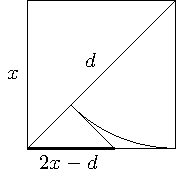
\includegraphics{images/euklid-quadrat}
    \caption{Euklids Konstruktoin}%
    \label{fig:euklid}
  \end{figure}

  Weiterhin gilt, dass sowohl $x_{1}$, als auch $d_{1}$, ganze Vielfache von $L$ sind:
  \begin{align*}
    x_{1} = d-x = (n-m)L \\
    d_{1} = 2x-d = (2m -n)L
  \end{align*}
  Nach Pythagoras gilt $d^{2} = 2x^{2}$, und somit $d \leq 3/2\cdot x$, da $(3/2)^{2} > 2$.
  Daraus folgt, dass
  \[x_{1} = d - x \leq \frac{1}{2} \cdot x.\]
  Iteriere dieses Verfahren und erhalte eine Serie von Quadraten mit Seiten
  $x_{2}, x_{3}, \dots$ und Diagonalen $d_{2}, d_{3}, \dots$. Es gilt:
  \[x_{k} \leq \frac{1}{2^{k}} \cdot x.\]
  Ausserdem ist jedes $x_{k}$ (und $d_{k}$) ein ganzes Vielfaches von $L$.
  Wähle nun $k$ so gross, dass
   \[x_{k} \leq \frac{1}{2^{k}} x < L.\]
   Dies impliziert, dass $x_{k} = 0$, was unmöglich ist. Deshalb können $x$ und $d$
   nicht kommensurabel sein.
\end{proof}

Wir haben diese Aussage mit einem sogenannten \textit{Widerspruchsbeweis} bewiesen.
Hierfür haben wir eine Annahme getroffen, und diese zu einem Widerspruch geführt.
Dies zeigt, dass unsere Annahme falsch war.

Wir sehen nun eine zeitgenössische Umformulierung dieses Antiken Resultats.
Seien $a,b > 0$ zwei kommensurable Längen. Das heisst, es existieren $L > 0$
und $m,n \in \mathbb N$ mit $a = mL$, $b= nL$. Dann gilt:
\[\frac{a}{b} = \frac{mL}{nL} = \frac{m}{n},\]
das heisst das Verhältnis $a/b$ ist eine \textit{rationale Zahl}.
Zurück zum Quadrat mit Seite $x$ und Diagonale $d$. Nach Pythagoras
gilt $d^{2} = 2x^{2}$. Falls $x=mL$ und $d=nL$ gilt,
dann also
\[2 = \frac{d^{2}}{x^{2}} = \left( \frac{d}{x}\right)^{2} = \left(\frac{n}{m}\right)^{2},\]
und somit
\[2m^{2} = n^{2}.\]
Die linke Seite dieser Gleichung ist durch $2$ teilbar. Dies impliziert, dass $n^{2}$, und
somit auch $n$, durch $2$ teilbar ist. Schreibe nun $n = 2k$. Schreibe $n = 2k$ mit
$k \in \mathbb N$. Setze ein und erhalte
$2m^{2} = (2k)^{2} = rk^{2}$,
beziehungsweise
\[m^{2} = 2k^{2}.\]
Die rechte Seite ist durch $2$ teilbar, also auch $m$.
Wir schliessen, dass sowohl $n$ als auch $m$ durch $2$ teilbar sind.
Schreibe noch $m = 2\ell$ mit $\ell \in \mathbb N$. Es gilt also
\[ 2 = \left(\frac{n}{m}\right)^{2}
  = \left(\frac{k}{\ell}\right)^{2}.\]
In anderen Worten sind Zähler und Nenner beide gerade.
Iteriere dieses Verfahren $k$ mal, bis $n/2^{k} < 1$, Dann entsteht ein Widerspruch.

\begin{corollary}
  Die Gleichung $z^{2} = 2$ hat keine rationale Lösung, das heisst,
  keine Lösung der Form $z = p/1$ mit $p, q \in \mathbb N$ und $q > 0$.
\end{corollary}

Das Ziel für den Rest dieses Kapitels ist es, eine Zahlenmenge $\mathbb R$ (die Menge
der \textit{reellen Zahlen}) zu konstruieren, in welcher die Gleichung
$z^{2} = 2$ eine Lösung hat.

\begin{exercise}
  Die Gleichung $z = \sqrt 2 x + \sqrt 3 y$ hat keine ganze Lösungen ausser $(0,0,0)$.
\end{exercise}
\end{document}
